\documentclass[11pt,a4paper]{article}

\usepackage[T1]{fontenc}
\usepackage[margin=1.7cm]{geometry}
\usepackage{amsmath,amssymb}
\usepackage{booktabs}
\usepackage{array}
\usepackage{xcolor}
\usepackage{listings}
\usepackage{tikz}
\usetikzlibrary{arrows.meta,positioning,shapes.geometric,calc}
\usepackage{hyperref}
\hypersetup{colorlinks=true,linkcolor=blue!50!black,citecolor=blue!50!black,urlcolor=blue!50!black}
\usepackage{enumitem}
\usepackage{titlesec}
\setlist{itemsep=1pt,topsep=3pt,parsep=1pt,partopsep=0pt}
\setlength{\abovecaptionskip}{3pt}
\setlength{\belowcaptionskip}{0pt}
\setlength{\textfloatsep}{6pt plus 2pt minus 2pt}
\setlength{\intextsep}{4pt plus 2pt minus 2pt}
\setlength{\abovedisplayskip}{4pt plus 1pt minus 2pt}
\setlength{\belowdisplayskip}{4pt plus 1pt minus 2pt}
\renewcommand{\arraystretch}{0.85}
\renewcommand{\paragraph}[1]{\par\smallskip\noindent\textbf{#1}}
\titlespacing*{\section}{0pt}{7pt}{3pt}
\titlespacing*{\subsection}{0pt}{5pt}{2pt}
\titlespacing*{\subsubsection}{0pt}{4pt}{2pt}
\linespread{0.97}
\setlength{\parskip}{0pt}

\lstdefinestyle{code}{
  basicstyle=\ttfamily\small,
  keywordstyle=\bfseries,
  commentstyle=\itshape\color{gray!70!black},
  stringstyle=\color{black},
  numbers=left,
  numberstyle=\tiny\color{gray},
  frame=single,
  breaklines=true,
  showstringspaces=false,
  tabsize=2,
  xleftmargin=1.5em,
  aboveskip=3pt,
  belowskip=0pt
}
\lstset{style=code}

\tikzset{
  box/.style={draw, rectangle, rounded corners, align=center, font=\small, text width=3.3cm, inner sep=2mm},
  subbox/.style={draw, rectangle, align=center, font=\footnotesize, text width=3.0cm, inner sep=1.5mm, fill=gray!8},
  note/.style={draw, rectangle, align=left, font=\footnotesize, text width=4.6cm, inner sep=1.5mm, fill=gray!8},
  decision/.style={draw, diamond, aspect=2, align=center, font=\footnotesize, inner sep=0.5mm, text width=2.3cm},
  arr/.style={-{Latex[length=2.2mm]}, thick},
  dashedline/.style={dashed, thin, gray!60!black}
}

\title{\textbf{A BDI--LLM Hybrid Multi-Agent System for DeliverooJS}}
\author{Davide Senette\\email: davide.senette@studenti.unitn.it, mat: 267070 \\\\Davide Sarti\\email: davide.sarti@studenti.unitn.it, mat: 267894}
\date{Autonomous Software Agents Course\\17 June 2026}

\begin{document}

\maketitle

% ============================================================
\section{System Overview}
\label{sec:overview}

\begin{description}
  \item[Agent A --- the LLM agent.] Runs an \emph{embedded} autonomous BDI loop
  (\texttt{startAutonomousBDI}) identical in implementation to Agent B's, and additionally
  listens on the chat channel. Each incoming chat message is interpreted by an LLM and executed
  through a tool-call loop (Section~\ref{sec:llm}). The embedded BDI keeps harvesting parcels
  with zero model calls while the LLM merely reads or queries state; it is paused only when a
  tool is about to take exclusive control of the agent's body (movement, delegated collection,
  rendezvous).
  \item[Agent B --- the BDI agent.] A pure reactive BDI agent with no LLM in its loop. It scores
  and executes intentions autonomously (Section~\ref{sec:scoring}) and can be \emph{preempted}
  by directives sent over the wire by Agent A (Section~\ref{sec:coordination}).
\end{description}

Both agents instantiate \texttt{createBeliefState()} (Section~\ref{sec:belief}) independently;
the two belief states are not a shared memory region but are kept consistent by an explicit
synchronization channel for persistent rules. The design separates four concerns that recur
throughout the codebase:

\begin{itemize}
  \item \textbf{Deliberation} --- option generation and scoring (\texttt{bdi/options.js},
  \texttt{bdi/bdiAgent.js}), independent of how an intention is eventually carried out.
  \item \textbf{Action execution} --- the plan layer (\texttt{actions/actions.js}), which turns
  a predicate into pathfinding and game-socket calls, falling back to PDDL when needed.
  \item \textbf{Coordination} --- a directive/status protocol (\texttt{bdi/coordination.js},
  \texttt{llm/coordinator.js}) layered on top of, but decoupled from, the scoring loop.
  \item \textbf{Shared beliefs} --- one schema (\texttt{beliefs/beliefState.js}) consumed
  identically by scoring, navigation, the LLM tools and the PDDL problem builder.
\end{itemize}

Figure~\ref{fig:architecture} shows the resulting data and control flow.

\begin{figure}[htbp]
\centering
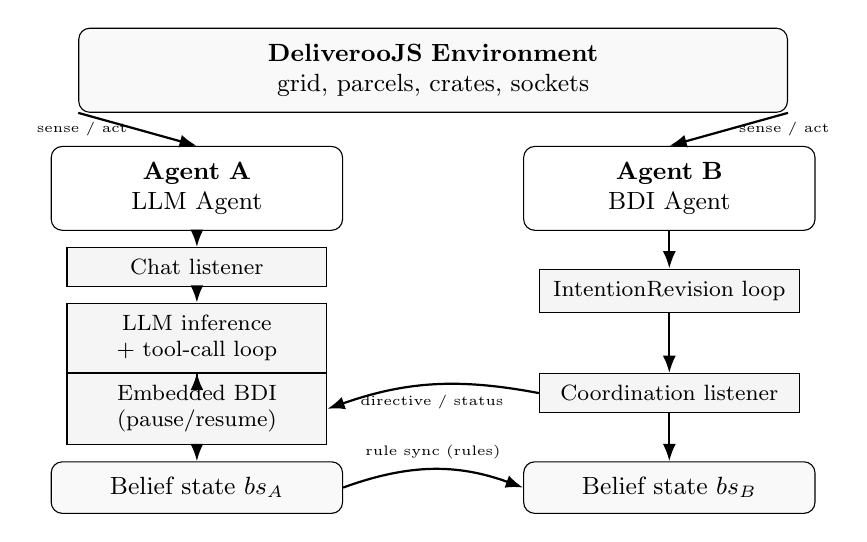
\begin{tikzpicture}[font=\footnotesize]
\node[box,text width=8.6cm,fill=gray!5] (env) at (4.3,7.6) {\textbf{DeliverooJS Environment}\\ grid, parcels, crates, sockets};

\node[box] (agentA) at (1.3,6.1) {\textbf{Agent A}\\ LLM Agent};
\node[box] (agentB) at (7.3,6.1) {\textbf{Agent B}\\ BDI Agent};

\node[subbox] (chat) at (1.3,5.1) {Chat listener};
\node[subbox] (llmloop) at (1.3,4.2) {LLM inference + tool-call loop};
\node[subbox] (ebdi) at (1.3,3.3) {Embedded BDI\\ (pause/resume)};
\node[box,fill=gray!5] (bsA) at (1.3,2.3) {Belief state $bs_A$};

\node[subbox] (bdiloop) at (7.3,4.8) {IntentionRevision loop};
\node[subbox] (coordlisten) at (7.3,3.5) {Coordination listener};
\node[box,fill=gray!5] (bsB) at (7.3,2.3) {Belief state $bs_B$};

\draw[arr] (env.south west) -- (agentA.north) node[midway,left,font=\tiny]{sense / act};
\draw[arr] (env.south east) -- (agentB.north) node[midway,right,font=\tiny]{sense / act};

\draw[arr] (agentA) -- (chat);
\draw[arr] (chat) -- (llmloop);
\draw[arr] (llmloop) -- (ebdi);
\draw[arr] (ebdi) -- (bsA);

\draw[arr] (agentB) -- (bdiloop);
\draw[arr] (bdiloop) -- (coordlisten);
\draw[arr] (coordlisten) -- (bsB);

\draw[arr] (bsA.east) to[bend left=20] node[midway,above,font=\tiny,text width=2.4cm,align=center]{rule sync (rules)} (bsB.west);
\draw[arr] (coordlisten.west) to[bend right=15] node[midway,below,font=\tiny,text width=2.6cm,align=center]{directive / status} (ebdi.east);
\end{tikzpicture}
\caption{Overall system architecture: two agents with structurally identical belief states,
connected by a rule-synchronization channel and a directive/status coordination channel. The
LLM agent's embedded BDI is the same code path as the standalone BDI agent's loop.}
\label{fig:architecture}
\end{figure}

% ============================================================
\section{Belief State}
\label{sec:belief}

\texttt{beliefs/beliefState.js} defines \texttt{createBeliefState()}, the single source of
truth read by option generation, scoring, navigation, the LLM tools and the PDDL problem
builder. No module keeps a parallel copy of world state; everything is derived from this
object on demand. Table~\ref{tab:belief-fields} summarizes its top-level sections.

\begin{table}[htbp]
\centering
\footnotesize
\begin{tabular}{@{}p{2.6cm}p{9.4cm}@{}}
\toprule
\textbf{Section} & \textbf{Content} \\
\midrule
\texttt{me} & \texttt{\{id, name, x, y, score\}} --- identity and current position. \\
\texttt{parcels}, \texttt{crates}, \texttt{agents} & \texttt{Map}s of sensed world objects keyed by id, refreshed on every sensing event. \\
\texttt{map} & \texttt{tiles}, \texttt{deliveryTiles}, \texttt{spawnTiles}, \texttt{pushableTiles} (type-5 / type-``5!'' tiles a crate can be pushed onto), \texttt{deliveryDistanceMap}, \texttt{spawnDistanceMap} (precomputed BFS distance tables, Section~\ref{sec:plans}), \texttt{grid}. \\
\texttt{config} & \texttt{observationDistance}, \texttt{movementDuration}, \texttt{playerCapacity}, \texttt{parcelDecayingEvent}, \texttt{parcelGenerationEvent}, \texttt{maxParcels} --- server-declared parameters. \\
\texttt{timing} & \texttt{decayTicks} (global counter of observed decay events) and \texttt{decayPerStep} (EMA of ticks per completed move, Section~\ref{sec:scoring}). \\
\texttt{rules} & Persistent strategy rules (Table~\ref{tab:rules-fields}), set only by the LLM agent's tools but mirrored onto the BDI agent's copy. \\
\texttt{coordination} & \texttt{active}, \texttt{queue}, \texttt{current}, \texttt{waiting}, \texttt{sendStatus}, \texttt{lastActivityMs} --- directive-mode state (Section~\ref{sec:coordination}). \\
\texttt{carry} & \texttt{\{count, campSteps\}} --- cached carried-parcel count and tiles patrolled while carrying in the current camp episode. \\
\texttt{lastParcelHint} & \texttt{\{x, y, ts\}} of the last tile where a parcel was \emph{actually picked up} (not merely sighted); anchors camping. \\
\bottomrule
\end{tabular}
\caption{Top-level sections of the belief state.}
\label{tab:belief-fields}
\end{table}

\begin{table}[htbp]
\centering
\footnotesize
\begin{tabular}{@{}p{3.0cm}p{9.0cm}@{}}
\toprule
\textbf{Field} & \textbf{Semantics} \\
\midrule
\texttt{stackSize} & Array of \texttt{\{mode, count, met, unmet\}}; several compatible constraints (e.g.\ \texttt{at\_least 2} and \texttt{at\_most 5}) coexist; conflicting ones are resolved at write time. \\
\texttt{parcelValueRules} & Array of \texttt{\{minReward, maxReward, mult, delta\}} value-band remaps applied at delivery time. \\
\texttt{penaltyDeliveries}, \texttt{preferredDeliveries} & \texttt{"x,y"} $\to$ \texttt{\{penalty\}} / \texttt{\{reward\}} maps for specific delivery tiles. \\
\texttt{deliveryMultipliers} & \texttt{"x,y"} $\to$ multiplier map for specific delivery tiles. \\
\texttt{penaltyTiles} & \texttt{"x,y"} $\to$ \texttt{\{penalty\}} map consumed by A* as a soft cost (\emph{not} a hard block). \\
\texttt{rendered} & Human/LLM-readable string derived from the structured fields, kept current by the rule tools. \\
\texttt{onChange} & Optional hook (wired by the LLM agent) fired after any rule mutation, used to push a full rule snapshot to the partner. \\
\bottomrule
\end{tabular}
\caption{Fields of \texttt{bs.rules}. All are soft preferences: they shift a score but, by
construction (Section~\ref{sec:scoring}), can never strand the agent without a viable
delivery or a passable route.}
\label{tab:rules-fields}
\end{table}

\paragraph{Object permanence.} Sensing is local and intermittent: a parcel or agent that leaves
observation range simply stops appearing in updates. Several belief-update paths therefore
treat the \emph{absence} of an expected entity as negative evidence rather than as silence,
combined with a short time-to-live: an agent's last known position
(\texttt{AGENT\_MEMORY\_TTL\_MS}, 3\,s) is retained briefly for the race-discount and soft-obstacle
computations and then dropped, so stale sightings do not bias scoring or pathfinding indefinitely.
The same TTL discipline applies to the avoided-tile memory used during navigation
(Section~\ref{sec:plans}): a tile that just refused a move is hard-avoided only for a few
move-durations, after which it becomes eligible again while the blocking agent is still in
sensing range.

% ============================================================
\section{Option Generation}
\label{sec:options}

\texttt{optionsGeneration(agent, bs)} (\texttt{bdi/options.js}) turns the current belief state
into a set of candidate predicates and inserts them into the intention queue in one batched
call. It is purely generative: it decides what is \emph{reachable}, never what is
\emph{worth doing} --- valuation is the exclusive responsibility of \texttt{intentionScore}
(Section~\ref{sec:scoring}).
\begin{table}[htbp]
\centering
\footnotesize
\begin{tabular}{@{}p{2.6cm}p{4.3cm}p{5.6cm}@{}}
\toprule
\textbf{Predicate} & \textbf{Generated when} & \textbf{Source} \\
\midrule
\texttt{go\_pick\_up x y id} & a free parcel has a finite pickup-route distance, and carried count $<$ effective capacity & one per visible free parcel \\
\texttt{go\_drop\_off x y} & at least one parcel is carried & one per delivery tile reachable from the current cell \\
\texttt{camp} & \texttt{AGENT\_CONFIG.behavior.camp} is enabled & single option, validity decided entirely in scoring \\
\texttt{explore} & always, as the idle fallback pushed directly by the loop & not generated here; pushed by \texttt{IntentionRevision.loop()} when the queue is empty \\
\bottomrule
\end{tabular}
\caption{Predicates produced by \texttt{optionsGeneration} (\texttt{explore} is pushed
separately by the idle branch of the revision loop, Section~\ref{sec:scoring}).}
\label{tab:options}
\end{table}

\texttt{agent.pushBatch(options)} filters out predicates already in the failed-intention
cooldown pool or already queued, inserts the rest, and re-sorts the queue exactly \emph{once}
regardless of batch size --- avoiding $O(n)$ re-sorts for $n$ newly generated options.

\texttt{optionsGeneration} returns immediately when \texttt{bs.coordination.active} is true: in
directive mode the BDI executes only what the LLM commands, so ordinary scored options must
neither compete with nor preempt the active coordination intention (Section~\ref{sec:coordination}).

% ============================================================
\section{Scoring and Intention Revision}
\label{sec:scoring}

\subsection{The IntentionRevision loop}

\texttt{IntentionRevisionRevise} (\texttt{bdi/bdiAgent.js}) maintains an intention queue and a
failed-intention cooldown pool (predicate $\to$ \texttt{\{addedAtMs, cooldownMs\}}, flat
\texttt{FAILED\_INTENTION\_RETRY\_MS} = 1\,s, no exponential backoff: a failure is almost
always transient congestion). Each pass of \texttt{loop()}:

\begin{enumerate}
  \item Idles if \texttt{paused} (an embedded owner, e.g.\ the LLM mission handler, is holding
  the body) or runs one coordination step if \texttt{coordination.active}.
  \item Re-queues failed intentions whose cooldown has elapsed.
  \item Drops the head intention if it has become structurally invalid (parcel already
  carried/gone, or no longer carrying anything for a queued delivery).
  \item Otherwise \texttt{achieve()}s the head intention, classifying the outcome as
  \emph{completed}, \emph{preempted}, \emph{failed} or \emph{stopped}, and reacts accordingly
  (Section~\ref{sec:failure}).
  \item Pushes \texttt{explore} when the queue is empty.
\end{enumerate}

\subsection{Score computation}

\texttt{intentionScore(predicate)} is the single authority on a predicate's worth; every number
below is computed fresh from \texttt{bs} at scoring time. The quantity represents the potential optimistic score gain from an action.

\paragraph{Decay factor.} Reward loss is priced through one quantity, the EMA-estimated reward
lost per carried parcel per tile traveled:
\begin{equation}
\text{factor} = \text{decayPerStep} =
\alpha \cdot \text{ticks}_t + (1-\alpha)\cdot \text{decayPerStep}_{t-1},
\qquad \alpha = 0.15
\label{eq:decay-ema}
\end{equation}
seeded by the config-derived prior $\text{movementDuration} / \text{decayInterval}$ and sampled
purely from server events (decay ticks observed between two consecutive move
acknowledgements), so it is immune to client load, network latency or server lag: a slower step
necessarily contains proportionally more ticks.

\paragraph{Drop-off score.} For \texttt{go\_drop\_off x y} with route distance $d$ (read from
\texttt{deliveryDistanceMap}) and carried parcels $p\in P$:
\begin{align}
\text{projected}_p &= \max(0,\, \text{reward}_p - d\cdot\text{factor}) \\
\text{banked}_p &= \text{projected}_p \cdot \text{mult}_v + \text{delta}_v
  \quad\text{(value-band remap, Section~\ref{sec:rulescoring})} \\
\text{sumBanked} &= -\text{DROP\_DISINCENTIVE} + \sum_{p\in P} \text{banked}_p \\
\text{scoreAfterStack} &= \text{sumBanked}\cdot\text{mult}_s + \text{delta}_s
  \quad\text{(stack delivery modifier at } |P| \text{)} \\
S_{\text{drop}}(x,y) &= \max\!\big(0,\ \text{scoreAfterStack}\cdot m(x,y) + r(x,y) - \pi(x,y)\big)
\label{eq:drop-score}
\end{align}
where $m,r,\pi$ are the tile's delivery multiplier, preferred reward and penalty
(\texttt{adjustDeliveryScore}). \texttt{DROP\_DISINCENTIVE} is currently 0.

\paragraph{Pickup score.} For \texttt{go\_pick\_up} of a new parcel $n$ with full route distance
$d$ (pickup leg $+$ nearest-delivery leg) and carried parcels $P$:
\begin{align}
\text{raceProb}(n) &= \frac{1}{1+\exp\!\big((d_{\text{me}\to n}-d_{\text{opp}\to n})/\tau\big)},
  \qquad \tau = \text{RACE\_DISCOUNT\_TAU} = 2
\label{eq:race-sigmoid} \\
\text{newDelivered} &= \Big(\max(0,\text{reward}_n - d\cdot\text{factor})\cdot\text{mult}_v+\text{delta}_v\Big)\cdot \text{raceProb}(n) \\
\text{carriedDelivered} &= \sum_{p\in P}\Big(\max(0,\text{reward}_p - d\cdot\text{factor})\cdot\text{mult}_{v,p}+\text{delta}_{v,p}\Big) \\
S_{\text{pick}}(n) &= \big(\text{carriedDelivered}+\text{newDelivered}\big)\cdot\text{mult}_{s}(|P|{+}1) + \text{delta}_{s}(|P|{+}1)
\label{eq:pickup-score}
\end{align}
The stack modifier in Eq.~\ref{eq:pickup-score} is evaluated \emph{optimistically} at the
resulting count $|P|{+}1$: gathering toward a target is priced with the rule's \texttt{met}
modifier, and only a pickup that \emph{overshoots} an \texttt{exactly}/\texttt{at\_most} cap
takes the \texttt{unmet} modifier (\texttt{stackPickupModifier}), so a sufficiently rich parcel
can still justify breaking the target stack. The race discount is applied \emph{after} the
value-band remap, never before: discounting first could push a high-value parcel into a
``worth 0'' band the moment any agent contests it.

\paragraph{Camp score.} \texttt{camp} is valid only while carrying ($|P|>0$), the harvest hint
is ``hot'', capacity remains, and no delivery tile is within
\texttt{CAMP\_NEAR\_DELIVERY\_TILES} = 8 (loitering near a delivery is never worth it: quick
cycles win). Patience is primarily spatial, then scaled by the server's declared spawn rate:
\begin{equation}
\text{patienceMs} = \operatorname{clamp}\!\big(\mu\cdot 1000\cdot(1.37^{\,n-3}-1),\,0,\,\mu\cdot 8000\big),
\qquad n=\min(n_{\text{adj}},10)
\label{eq:camp-patience}
\end{equation}
forced to 0 when $n_{\text{adj}} < 4$ or the server declares infinite parcel generation, with
$n_{\text{adj}}$ the number of spawn tiles within Manhattan radius 3 of the harvest anchor (the
constants are \texttt{CAMP\_PATIENCE\_MIN\_TILES}=4 and \texttt{CAMP\_PATIENCE\_SATURATION\_TILES}=10)
and $\mu=\min\!\big(\text{CAMP\_SPAWN\_RATE\_MAX\_MULT},\,\max$\\$(1,\,\text{CAMP\_SPAWN\_RATE\_NEUTRAL\_MS}/\text{parcelGenerationEvent})\big)$,
\texttt{CAMP\_SPAWN\_RATE\_MAX\_MULT}=1.3 and \texttt{CAMP\_SPAWN\_RATE\_NEUTRAL\_MS}=2000\,ms, so a
map that spawns faster than the 2\,s neutral rate stretches both the growth curve and its ceiling,
making a hot pocket worth camping longer. While hot, the camp loss
budget bounds how long camping is worth it relative to delivering now:
\begin{equation}
\text{horizon} = \frac{\max\big(\text{CAMP\_LOSS\_BUDGET\_FRACTION}\cdot\text{totalReward},\ \text{stackCampGain}\big)}{\text{factor}\cdot|P|}
\label{eq:camp-horizon}
\end{equation}
where \texttt{stackCampGain} is the extra delivery value reachable by gathering more parcels up
to an active stack-rule target (0 when no rule, or when the cap is already exceeded and cannot
be undone by waiting). Camp is invalid once \texttt{campSteps} $\geq$ horizon. When valid:
\begin{equation}
S_{\text{camp}} = \text{totalReward} + \text{CAMP\_INCENTIVE},\qquad \text{CAMP\_INCENTIVE}=0.02
\label{eq:camp-score}
\end{equation}
which deliberately outranks a plain delivery of the same load (so the agent gathers a fuller
load first) but stays below any real pickup (\(\text{totalReward}+\text{reward}_n\)), so a
visible parcel is still grabbed before camping is reconsidered.

\paragraph{Exploration score.} A flat floor, $S_{\text{explore}} = \text{EXPLORATION\_INCENTIVE} = 0.01$,
strictly below camp so an idle agent prefers to camp a hot pocket over wandering, but high
enough to keep the agent moving when nothing else scores positively.

\subsubsection{Persistent-rule modifiers}
\label{sec:rulescoring}

\texttt{bdi/ruleScoring.js} implements the rule effects referenced above as pure functions of
\texttt{bs.rules}, kept independent of the scoring loop so they cannot silently diverge from it:

\begin{itemize}
  \item \textbf{Parcel value bands.} Each rule \texttt{\{minReward,maxReward,mult,delta\}}
  contributes its modifier when a value $v$ lies in $[\text{minReward},\text{maxReward}]$
  (open bounds), combined multiplicatively/additively across overlapping rules:
  $v' = v\cdot\!\prod\text{mult}_i + \sum\text{delta}_i$.
  \item \textbf{Stack-size combination.} \texttt{combineStack} multiplies every active rule's
  chosen modifier (\texttt{met} or \texttt{unmet}, selected per-context) and sums the deltas;
  two rules \emph{conflict} (and the older is dropped on write) exactly when their
  satisfied-count ranges --- $[N,\infty)$ for \texttt{at\_least}, $[1,N]$ for \texttt{at\_most},
  $[N,N]$ for \texttt{exactly} --- do not overlap.
  \item \textbf{Delivery-tile preferences.} $\text{adjusted} = \max(0,\ \text{base}\cdot m + r - \pi)$
  (Eq.~\ref{eq:drop-score}); the floor at 0 is what keeps a penalty a pure \emph{reordering}
  device rather than a way to forbid the agent's only path to banking reward.
\end{itemize}

Table~\ref{tab:constants} collects the numeric constants governing scoring and preemption.

\begin{table}[htbp]
\centering
\footnotesize
\begin{tabular}{@{}llp{7.2cm}@{}}
\toprule
\textbf{Constant} & \textbf{Value} & \textbf{Role} \\
\midrule
\texttt{HOARD\_CAP} & 10 & Hard ceiling on carried parcels regardless of server-declared capacity. \\
\texttt{RACE\_DISCOUNT\_TAU} & 2 tiles & Sigmoid temperature in Eq.~\ref{eq:race-sigmoid}. \\
\texttt{PREEMPTION\_HYSTERESIS} & 0.25 & Relative margin a challenger must clear (Section~\ref{sec:hysteresis}). \\
\texttt{PREEMPTION\_EPSILON} & 0.001 & Additive margin guarding against float-equality ties. \\
\texttt{CAMP\_NEAR\_DELIVERY\_TILES} & 8 & Distance below which camping is disabled in favor of delivering. \\
\texttt{CAMP\_LOSS\_BUDGET\_FRACTION} & 0.05 & Fraction of carried reward camping may bleed to decay. \\
\texttt{EXPLORATION\_INCENTIVE} & 0.01 & Flat exploration floor. \\
\texttt{CAMP\_INCENTIVE} & 0.02 & Flat margin by which camp outranks an equal-value delivery. \\
\texttt{FAILED\_INTENTION\_RETRY\_MS} & 1000\,ms & Flat cooldown before a failed predicate is re-probed. \\
\bottomrule
\end{tabular}
\caption{Scoring and preemption constants (\texttt{utils/constants.js}, \texttt{bdi/options.js}).}
\label{tab:constants}
\end{table}

\subsection{Hysteresis preemption}
\label{sec:hysteresis}

\texttt{sortQueueByScore()} re-scores every queued intention, drops any with score $\leq 0$ (so
a hard-forbidden delivery, floored to 0 by Eq.~\ref{eq:drop-score}, naturally leaves the queue),
and re-sorts by descending score. Switching the \emph{running} intention is not free --- a
half-walked route has a real sunk cost --- so a challenger must clear a hysteresis band:
\begin{equation}
S_{\text{challenger}} \;>\;
\begin{cases}
S_{\text{running}}\,(1+h) + \varepsilon & \text{if } S_{\text{running}} > 0 \\
0 & \text{if } S_{\text{running}} \leq 0
\end{cases}
\label{eq:hysteresis}
\end{equation}
with $h=0.25$ and $\varepsilon=0.001$ (Table~\ref{tab:constants}); an already-invalid running
intention ($S_{\text{running}}\leq 0$) is abandoned immediately. This protects deliveries in final approach naturally: the drop-off score in
Eq.~\ref{eq:drop-score} \emph{peaks} right before the tile (route distance $\to 0$), so the bar
for interruption is highest exactly where switching would waste the most progress. A
\texttt{committedManeuver} flag (set while a PDDL crate-push is in flight, Section~\ref{sec:pddl})
unconditionally disables preemption: restarting a partial push from scratch would waste the
detour already taken to get behind the crate.

When preemption fires, the running intention is \texttt{stop(STOP\_REASON\_PREEMPTION)}'d; its
\texttt{achieve()} promise rejects with a tagged \emph{preempted} error, and the loop
\textbf{requeues} a fresh \texttt{Intention} for the same predicate (not failed, not
cooled down) so it competes again on the next sort.

\subsection{Failure handling}
\label{sec:failure}

\begin{table}[htbp]
\centering
\footnotesize
\begin{tabular}{@{}p{2.4cm}p{9.9cm}@{}}
\toprule
\textbf{Outcome} & \textbf{Handling} \\
\midrule
\textit{completed} & Intention removed from the queue; no special action. \\
\textit{preempted} & Re-queued as a fresh intention (Section~\ref{sec:hysteresis}); never enters the cooldown pool. \\
\textit{failed} & Added to the failed-intention pool for \texttt{FAILED\_INTENTION\_RETRY\_MS}; if the failed predicate was \texttt{go\_drop\_off}, \texttt{\#pushNextNearestDelivery} immediately queues the next-nearest \emph{other} delivery tile so the agent is never left with zero delivery options while parcels keep decaying. \\
\textit{stopped} & A clean, non-preemption stop (e.g.\ a manual pause or a propagated \texttt{["stopped"]}); removed without cooldown or replacement. \\
\bottomrule
\end{tabular}
\caption{Intention outcomes and their effect on the queue.}
\label{tab:outcomes}
\end{table}

Figure~\ref{fig:revision-cycle} summarizes the full cycle.

\begin{figure}[htbp]
\centering
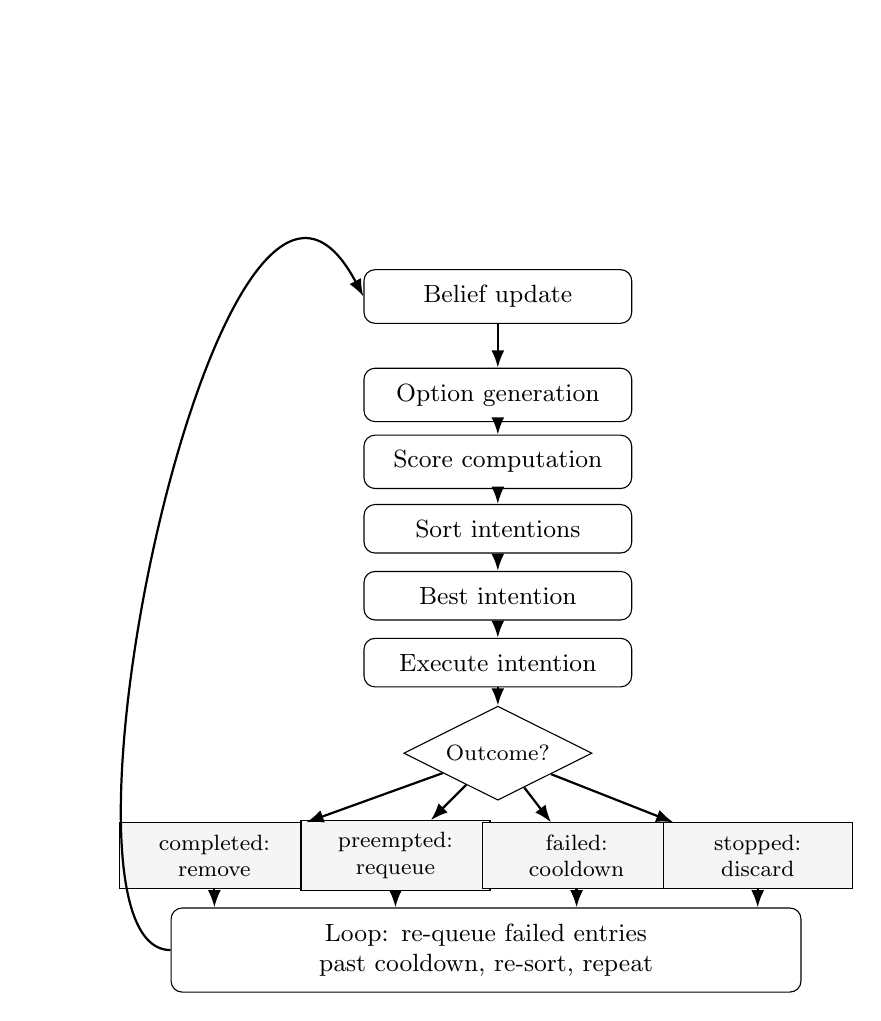
\begin{tikzpicture}[font=\footnotesize]
\node[box,text width=3.0cm] (belief) at (4,8.1) {Belief update};
\node[box,text width=3.0cm] (optgen) at (4,6.85) {Option generation};
\node[box,text width=3.0cm] (score) at (4,6) {Score computation};
\node[box,text width=3.0cm] (sort) at (4,5.15) {Sort intentions};
\node[box,text width=3.0cm] (best) at (4,4.3) {Best intention};
\node[box,text width=3.0cm] (exec) at (4,3.45) {Execute intention};
\node[decision,text width=1.7cm] (outcome) at (4,2.3) {Outcome?};

\node[subbox,text width=2.1cm] (completed) at (0.4,1.0) {completed: remove};
\node[subbox,text width=2.1cm] (preempted) at (2.7,1.0) {preempted: requeue};
\node[subbox,text width=2.1cm] (failed) at (5.0,1.0) {failed: cooldown};
\node[subbox,text width=2.1cm] (stopped) at (7.3,1.0) {stopped: discard};

\node[box,text width=7.6cm] (loopback) at (3.85,-0.2) {Loop: re-queue failed entries past cooldown, re-sort, repeat};

\draw[arr] (belief) -- (optgen);
\draw[arr] (optgen) -- (score);
\draw[arr] (score) -- (sort);
\draw[arr] (sort) -- (best);
\draw[arr] (best) -- (exec);
\draw[arr] (exec) -- (outcome);

\draw[arr] (outcome) -- (completed);
\draw[arr] (outcome) -- (preempted);
\draw[arr] (outcome) -- (failed);
\draw[arr] (outcome) -- (stopped);

\draw[arr] (completed) -- (loopback.north -| completed);
\draw[arr] (preempted) -- (loopback.north -| preempted);
\draw[arr] (failed) -- (loopback.north -| failed);
\draw[arr] (stopped) -- (loopback.north -| stopped);

\draw[arr] (loopback.west) .. controls +(-1.8,0) and +(-1.8,3.4) .. (belief.west);
\end{tikzpicture}
\caption{Intention revision cycle. The sort step (Eq.~\ref{eq:hysteresis}) is where hysteresis
preemption is decided; the four outcomes feed back into the same loop via the failed-intention
pool and the delivery fallback of Section~\ref{sec:failure}.}
\label{fig:revision-cycle}
\end{figure}

% ============================================================
\section{Plans and Navigation}
\label{sec:plans}

\texttt{executePredicate} (\texttt{actions/actions.js}) is the one entry point translating a
predicate into game-socket calls; it is shared verbatim by the autonomous loop, the
coordination layer and the LLM's delegated tools.

\begin{table}[htbp]
\centering
\footnotesize
\begin{tabular}{@{}p{2.4cm}p{9.9cm}@{}}
\toprule
\textbf{Predicate} & \textbf{Behavior} \\
\midrule
\texttt{go\_to x y} & A*-routes to $(x,y)$, replanning on a blocked step (up to \texttt{MAX\_REPLANS}=3) and falling back to PDDL when a crate is the sole blocker. \\
\texttt{go\_pick\_up x y id} & \texttt{go\_to} then \texttt{pickup()}; records \texttt{lastParcelHint} on a successful grab. \\
\texttt{go\_drop\_off x y} & \texttt{go\_to} then \texttt{putdown()}; increments \texttt{bs.metrics.deliveredParcels} only when the tile is a genuine delivery tile (a handoff drop on a plain tile banks nothing). \\
\texttt{explore} & \texttt{go\_to} on the least-recently-visited reachable spawn tile (\texttt{findCellsToExplore}, distance/staleness weighted). \\
\texttt{camp} & Patrols the perimeter of the spawn cluster around the harvest anchor (Section~\ref{sec:scoring}), charging \texttt{carry.campSteps}. \\
\texttt{go\_near x y maxDist} & \texttt{go\_to} on the closest reachable tile inside the Manhattan diamond of radius \texttt{maxDist} around $(x,y)$; used by rendezvous. \\
\texttt{wait signal timeoutMs} & Blocks until \texttt{bs.coordination.waiting} is cleared by an incoming \texttt{signal} message, or until an optional timeout; default is unbounded. \\
\bottomrule
\end{tabular}
\caption{Plan predicates dispatched by \texttt{executePredicate}.}
\label{tab:plans}
\end{table}

\paragraph{Navigation principles.}
\begin{itemize}
  \item \textbf{A* with mixed hard/soft obstacles.} Walls and crates are hard; other agents are
  hard only within \texttt{SOFT\_OBSTACLE\_HARD\_RADIUS}=1 tiles of the start (they are
  genuinely in the way \emph{now}), and merely add \texttt{AGENT\_SOFT\_PENALTY}=7.5 to the edge
  cost otherwise (they will likely have moved by the time the agent arrives).
  \item \textbf{Soft penalties from rules.} Entering a tile in \texttt{bs.rules.penaltyTiles}
  costs extra (added to \texttt{BASE\_STEP\_COST}=1) but is never refused, so an LLM navigation
  rule can steer the route without ever stranding the agent.
  \item \textbf{Adaptive timeout.} $\text{timeout} = \max(\text{GO\_TO\_TIMEOUT\_MS},\ |\text{path}|\cdot\text{movementDurationMs}\cdot\text{GO\_TO\_TIMEOUT\_SAFETY\_FACTOR})$,
  with \texttt{GO\_TO\_TIMEOUT\_SAFETY\_FACTOR}=3, so short legs fail fast and long legs are not spuriously timed out.
  \item \textbf{\texttt{avoidTiles}.} A tile that just physically refused a move is hard-blocked
  for \texttt{AVOID\_TENURE\_MOVE\_FACTOR}=3 move-durations, forcing the replanner onto a
  genuinely different route instead of greedily re-entering a proven choke; the memory expires
  quickly so a cleared corridor is retried while still in sensing range.
  \item \textbf{Opportunistic pickup and delivery.} \texttt{opportunisticActions()} runs after
  every step: it grabs a free, rule-eligible parcel standing on the just-entered tile (zero
  detour) and auto-banks carried parcels on a delivery tile, unless a stack rule is still
  unmet or the tile is penalised --- suspended entirely while \texttt{coordination.active}.
  \item \textbf{BFS distance maps.} \texttt{deliveryDistanceMap} and \texttt{spawnDistanceMap}
  are precomputed once per tile (multi-source shortest-path tables) so route-distance lookups
  used throughout scoring (Eqs.~\ref{eq:drop-score}--\ref{eq:pickup-score}) are $O(1)$ instead of
  re-running BFS/A* on every score evaluation.
  \item \textbf{Crate detection.} \texttt{crateBlocksRoute()} plans twice --- once respecting
  crates, once with \\ \texttt{ignoreCrates:true} --- and concludes a crate is the blocker only when
  the first fails and the second succeeds, avoiding false positives from an agent merely
  orbiting a temporarily occupied choke.
  \item \textbf{PDDL invocation.} On a confirmed crate block, \texttt{pddlReach} sets
  \texttt{bs.committedManeuver=true}, solves and executes a push plan (Section~\ref{sec:pddl}),
  and clears the flag in a \texttt{finally}, regardless of outcome.
\end{itemize}

% ============================================================
\section{The LLM Layer}
\label{sec:llm}

\subsection{Architecture}

\texttt{startLLMAgent(socket, bs, llmState, actions)} wires three independent pieces onto one
agent: an embedded autonomous BDI (\texttt{startAutonomousBDI}, identical code path to Agent B),
a \texttt{createCoordinator} for talking to the partner, and a chat listener. Incoming chat
messages are pushed through \\ \texttt{createMissionQueue}, which serializes mission handling so
two rapid messages never race over the same pause/resume state or the same parcels.

Pausing is \emph{lazy}: the embedded BDI keeps harvesting while the LLM reasons about a message,
and is paused only the first time a body-controlling tool (Table~\ref{tab:bdi-pausing}) is about
to execute, via \texttt{pauseBdiForMission()} (idempotent, guarded by \texttt{pausedForMission}).
A pure rule/query mission therefore never interrupts ongoing play. The \texttt{finally} block
unconditionally calls \texttt{bdi.resume()} at mission end, \emph{unless} the agent was
deliberately parked on an external signal (\texttt{partnerParkedOn} set, Section~\ref{sec:coordination}),
in which case the next mission turn must relay that signal before resuming.

\begin{table}[htbp]
\centering
\footnotesize
\begin{tabular}{@{}p{6.0cm}p{6.0cm}@{}}
\toprule
\textbf{Pauses the embedded BDI} & \textbf{Does not pause it} \\
\midrule
\texttt{collect\_and\_deliver}, \texttt{go\_to}, \texttt{go\_pick\_up}, \texttt{go\_drop\_off},
\texttt{rendezvous\_with\_partner}, \texttt{handoff\_to\_partner}, \texttt{wait\_for\_partner} &
\texttt{observe\_environment}, \texttt{calculate}, every rule/navigation store tool,
\texttt{direct\_partner}, \texttt{signal\_partner} \\
\bottomrule
\end{tabular}
\caption{\texttt{BDI\_PAUSING\_TOOLS}: only tools that take exclusive control of this agent's
own body (or must hold it still for a teammate) pause the embedded loop.}
\label{tab:bdi-pausing}
\end{table}

\subsection{Prompt engineering}

The system prompt (\texttt{SYSTEM\_EXECUTOR\_PROMPT}) is organized as a strict decision
procedure, not free-form instructions:

\begin{description}
  \item[Role / output contract.] Exactly one tool call per step; the loop continues until
  \texttt{final\_reply}.
  \item[Reward phrasing.] Any mission tying points to an outcome (``+N pts if X'') is reframed
  as motivation, never as a passive fact: it resolves either to a durable RULE or to an active
  TASK, never to a no-op.
  \item[Rejection whitelist.] A \emph{closed} list of four grounds --- unresolved coordinate
  placeholder, explicit negative immediate reward, violation of an active persistent rule, or
  genuinely garbled text. Everything else must be classified and acted on; the prompt explicitly
  forbids inventing further rejection reasons (vagueness, missing specifics, future tense).
  \item[Anti-hallucination.] The model may only use parcels/tiles/rewards present in the
  supplied state or a fresh \texttt{observe\_environment} call --- never invented.
  \item[Mission classification.] Every mission is first sorted into RULE, TASK or QUERY; the
  prompt calls this ``the most common mistake'' and forces the decision before any tool call.
  \item[Compound missions.] A boolean \texttt{more} flag on terminal tools lets ``do X AND do
  Y'' missions chain multiple terminal calls without ending after the first clause.
  \item[Team coordination rules.] Eight numbered rules disambiguating solo vs.\ team missions,
  when to use \texttt{rendezvous\_with\_partner} versus manual \texttt{direct\_partner} +
  \texttt{wait\_for\_partner}, and the asymmetric handoff protocol (Section~\ref{sec:coordination}).
  \item[Few-shot examples.] \texttt{EXECUTOR\_EXAMPLES} enumerates $\sim$20 worked
  mission$\to$tool-sequence pairs covering rejections, factual queries, durable rules (including
  compound and replacement cases), harvesting tasks, rendezvous and handoffs --- each annotated
  with the reasoning that produced the sequence.
\end{description}

\subsection{Tool catalog}

\begin{table}[htbp]
\centering
\footnotesize
\begin{tabular}{@{}p{3.0cm}p{9.0cm}@{}}
\toprule
\textbf{Category} & \textbf{Tools} \\
\midrule
Self-action & \texttt{move\_to}, \texttt{pick\_up\_parcel}, \texttt{deliver\_carried\_parcels}, \texttt{collect\_and\_deliver} (delegates to the embedded BDI, Section~\ref{sec:llm-exec-loop}) \\
Query & \texttt{observe\_environment}, \texttt{calculate}, \texttt{resolve\_delivery\_tile} \\
Coordination & \texttt{rendezvous\_with\_partner}, \texttt{handoff\_to\_partner}, \texttt{direct\_partner}, \texttt{signal\_partner}, \texttt{wait\_for\_partner} \\
Persistent rules & \texttt{set\_stack\_size\_rule}, \texttt{remove\_stack\_size\_rule}, \texttt{set\_parcel\_value\_rule}, \texttt{remove\_parcel\_value\_rule}, \texttt{forbid\_delivery\_tile}, \texttt{prefer\_delivery\_tile}, \texttt{set\_delivery\_tile\_multiplier}, \texttt{remove\_delivery\_tile\_rule}, \texttt{clear\_durable\_rules}, \texttt{block\_navigation\_tile}, \texttt{unblock\_navigation\_tile}, \texttt{clear\_navigation\_rules} \\
\bottomrule
\end{tabular}
\caption{Tool catalog exposed to the executor LLM (\texttt{SYSTEM\_EXECUTOR\_TOOLS}).}
\label{tab:tools}
\end{table}

\subsection{Execution loop}
\label{sec:llm-exec-loop}

For each chat message, a fresh \texttt{[system, user]} message pair is built --- the system
prompt plus a user prompt embedding the raw mission text, the rendered rule set, and a validator
snapshot of the current game state. The loop (capped at \texttt{MAX\_ITERATIONS}=100) repeats:

\begin{enumerate}
  \item Call the model with \texttt{temperature=0} and the full tool list; strip the
  control-flow fields \texttt{thought} and \texttt{more} before forwarding parameters to the
  tool implementation.
  \item \texttt{mapExecutorAction} translates the executor's tool name/shape into the internal
  action used by \texttt{executeTool} (e.g.\ \texttt{pick\_up\_parcel} $\to$ \texttt{go\_pick\_up}).
  \item \texttt{validateActionAgainstPersistentRules} checks the action against active rules
  \emph{before} execution; a violation is fed back as a tool observation so the model can pick a
  different step, without ever running the disallowed action.
  \item If the action is in \texttt{BDI\_PAUSING\_TOOLS}, pause the embedded BDI (once).
  \item Execute the tool, append its observation as a \texttt{tool} message.
  \item \textbf{Terminal tools} (every persistent-rule/navigation store, plus
  \texttt{collect\_and\_deliver} via \\ \texttt{toolResult.terminal}) end the mission immediately
  on success, using the tool's own confirmation text as the chat reply --- saving the extra
  round-trip a separate \texttt{final\_reply} would cost --- \emph{unless} the tool errored or
  \texttt{more:true} was set for a remaining compound clause.
  \item \texttt{final\_reply} always ends the mission with an explicit message.
\end{enumerate}

Concretely, for ``collect three parcels and deliver them'': the chat message enters the mission
queue, the LLM emits a single \texttt{collect\_and\_deliver(parcels=3)} tool call, the embedded
BDI is unpaused and watches \texttt{deliveredParcels} climb with zero further model calls, and
once the target is reached (or the time budget elapses) the tool returns and the BDI is
re-paused, ending the mission in one model round-trip.

% ============================================================
\section{Multi-Agent Coordination}
\label{sec:coordination}

Coordination is a thin asynchronous protocol over the SDK's \texttt{say} channel
(\texttt{utils/coordProtocol.js}), layered on top of, but not replacing, each agent's ordinary
intention queue.

\begin{table}[htbp]
\centering
\footnotesize
\begin{tabular}{@{}p{2.0cm}p{1.6cm}p{8.7cm}@{}}
\toprule
\textbf{Message} & \textbf{Direction} & \textbf{Payload / effect} \\
\midrule
\texttt{directive} & LLM$\to$BDI & \texttt{\{cid, command, args\}}; queued and, on arrival, preempts the BDI's running intention via \texttt{preemptForCoordination()}. \\
\texttt{status} & BDI$\to$LLM & \texttt{\{cid, ok, detail\}}; resolves the matching \texttt{wait\_for\_partner}, or is buffered if none is waiting yet. \\
\texttt{signal} & LLM$\to$BDI & \texttt{\{signal\}}; out-of-band release of \texttt{bs.coordination.waiting}. \\
\texttt{rules} & LLM$\to$BDI & Full serialized rule snapshot (idempotent; a missed update self-heals on the next change), applied via \texttt{applyRulesSnapshot}. \\
\bottomrule
\end{tabular}
\caption{Coordination protocol messages (\texttt{COORD\_PROTO="coord"}).}
\label{tab:coord-messages}
\end{table}

\paragraph{Coordinator side (\texttt{llm/coordinator.js}).} \texttt{pendingWaiters} (cid
$\to$ resolver) and \texttt{bufferedStatuses} (cid $\to$ status) together make
\texttt{directPartner}/\texttt{waitForPartner} order-independent: a status that arrives before
anyone waits for it is buffered and consumed by the next matching \texttt{waitForPartner}.
\texttt{syncRules} fires automatically from \texttt{bs.rules.onChange}, so the BDI-only partner's
copy of \texttt{bs.rules} never drifts from the LLM's.

\paragraph{BDI side (\texttt{bdi/coordination.js}).} \texttt{setupBdiCoordination} attaches a
message listener that pushes directives into \texttt{bs.coordination.queue}, flips
\texttt{active}, and calls \texttt{agent.preemptForCoordination()}. \\ \texttt{\#runCoordination()}
then drains the queue one directive at a time: \texttt{coordToPredicate} maps the wire command
onto the same predicates Table~\ref{tab:plans} describes so directive execution reuses the ordinary plan layer verbatim.
\texttt{vacateAfterDrop()} steps the agent one tile off its cell after a \texttt{putdown} so the
partner can physically occupy the just-vacated tile to collect the handoff parcel. A
\texttt{resume} directive clears \texttt{coordination.active}, returning control to the scored
loop; an idle TTL (\texttt{COORD\_RESUME\_IDLE\_TTL\_MS}=15\,s) auto-resumes defensively if the
LLM partner disappears mid-directive.

\paragraph{Handoff protocol.} A cross-delivery handoff is driven end-to-end by a single tool,
\texttt{handoff\_to\_partner}, rather than by the model manually sequencing
\texttt{direct\_partner}/\texttt{wait\_for\_partner} calls. The tool: (1) repeatedly issues
\texttt{direct\_partner(pickup)} with no coordinates so the BDI self-selects via
\texttt{\#selectBestPickup()} (reusing \texttt{intentionScore}, so it never diverges from normal
play), stacking up to an optional target count or a safety cap (\texttt{HANDOFF\_MAX\_PICKUPS});
(2) sends \texttt{direct\_partner(go\_near)} to bring the loaded BDI adjacent to the LLM agent
before dropping, so the hand-off lands within trivial reach; (3) issues
\texttt{direct\_partner(putdown)} at the BDI's own (now-adjacent) cell and waits for
\texttt{status(ok)}, sent only after \texttt{vacateAfterDrop()} has stepped the BDI off the tile;
(4) walks the LLM agent onto the vacated tile and retries the pickup a few times. (5) By
default delivers the collected load to the nearest delivery tile and reports the parcels
actually banked.

\paragraph{Rendezvous / barrier synchronization.} \texttt{rendezvous\_with\_partner} sends
\texttt{go\_near} to the partner, moves the LLM agent itself in parallel, then waits for both
arrivals before releasing the partner with \texttt{resume} --- a single atomic barrier that
avoids the race window a manual direct/move/wait sequence would leave open.

\begin{figure}[htbp]
\centering
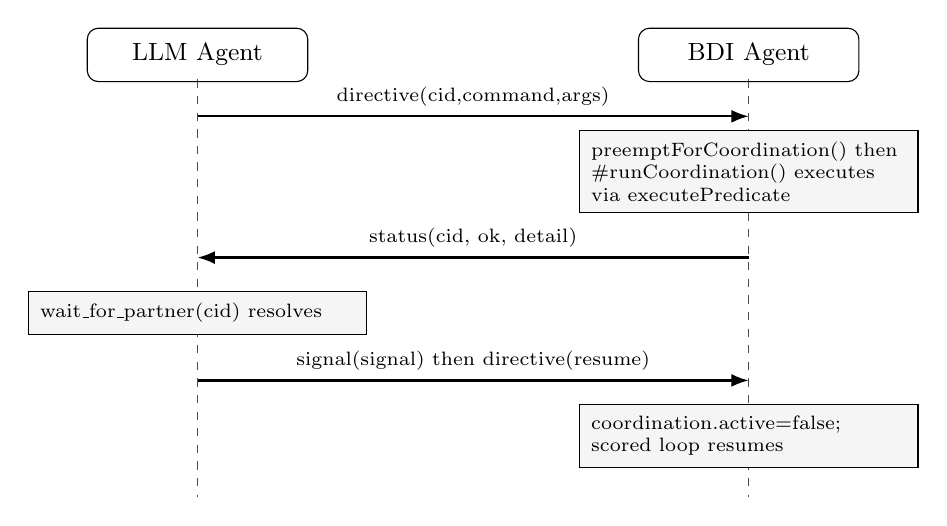
\begin{tikzpicture}[yscale=0.78]
\draw[dashedline] (2,6.8) -- (2,0);
\draw[dashedline] (9,6.8) -- (9,0);
\node[box,text width=2.4cm] (llmlife) at (2,7.2) {\small LLM Agent};
\node[box,text width=2.4cm] (bdilife) at (9,7.2) {\small BDI Agent};

\draw[arr] (2,6.2) -- (9,6.2) node[midway,above,font=\scriptsize]{directive(cid,command,args)};
\node[note,text width=4.0cm,font=\scriptsize] at (9,5.3) {preemptForCoordination() then \#runCoordination() executes via executePredicate};
\draw[arr] (9,3.9) -- (2,3.9) node[midway,above,font=\scriptsize]{status(cid, ok, detail)};
\node[note,text width=4.0cm,font=\scriptsize] at (2,3.0) {wait\_for\_partner(cid) resolves};
\draw[arr] (2,1.9) -- (9,1.9) node[midway,above,font=\scriptsize]{signal(signal) then directive(resume)};
\node[note,text width=4.0cm,font=\scriptsize] at (9,1.0) {coordination.active=false; scored loop resumes};
\end{tikzpicture}
\caption{Multi-agent coordination protocol. Cross arrows are wire messages; boxed notes are
local actions taken on receipt. The same exchange, with \texttt{pickup}/\texttt{putdown}
commands, implements the asymmetric parcel handoff described above.}
\label{fig:coord-protocol}
\end{figure}

% ============================================================
\section{PDDL}
\label{sec:pddl}

When A* reports that a route is blocked and \texttt{crateBlocksRoute()} confirms a crate is the
sole obstacle, the agent falls back to a STRIPS planner (\texttt{pddl/domain.pddl}) capable of
pushing crates aside --- a maneuver A* cannot express.

\begin{table}[htbp]
\centering
\footnotesize
\begin{tabular}{@{}p{3.4cm}p{8.6cm}@{}}
\toprule
\textbf{Predicate} & \textbf{Meaning} \\
\midrule
\texttt{(tile ?t)} & \texttt{?t} is a walkable cell (walls, type 0, are excluded entirely). \\
\texttt{(free ?t)} & No agent and no crate on \texttt{?t} (parcels never block). \\
\texttt{(delivery ?t)}, \texttt{(pushable ?t)} & Delivery zone / type-5 crate-receiving tile. \\
\texttt{(up/down/left/right ?from ?to)} & Directional adjacency, emitted only between two existing tiles. \\
\texttt{(at-agent ?t)} & Current agent position. \\
\texttt{(parcel ?p)}, \texttt{(at-parcel ?p ?t)}, \texttt{(carrying ?p)}, \texttt{(delivered ?p)} & Parcel type guard, floor position, carried state, terminal delivered state. \\
\texttt{(crate ?c)}, \texttt{(at-crate ?c ?t)} & Crate type guard and position. \\
\bottomrule
\end{tabular}
\caption{Domain predicates (\texttt{pddl/domain.pddl}).}
\label{tab:pddl-predicates}
\end{table}

\textbf{Actions:} four \texttt{move-*} actions, one per direction (precondition: the adjacent
tile in that direction is free), and four matching \texttt{push-*} actions, which move the agent
onto the crate's tile while sliding the crate one step further in the same direction onto a
\texttt{pushable} tile that is \texttt{free}. At execution time both collapse to the same
primitive: the server has no separate push command, so moving \emph{into} a crate that has a
clear type-5 tile behind it pushes it automatically (\texttt{planExecutor.js}'s
\texttt{ACTION\_MAP} maps every \texttt{push-*} action to \texttt{actions.move(direction)}).

\begin{lstlisting}[language={},caption={Push action (excerpt, \texttt{pddl/domain.pddl}): the
agent and the crate must be co-linear in the push direction, and the destination must be both
\texttt{free} and \texttt{pushable}.},label={lst:pddl-push}]
(:action push-right
  :parameters (?c ?agentPos ?cratePos ?destPos)
  :precondition (and (crate ?c) (at-agent ?agentPos)
    (at-crate ?c ?cratePos) (right ?agentPos ?cratePos)
    (right ?cratePos ?destPos)
    (free ?destPos) (pushable ?destPos))
  :effect (and (at-agent ?cratePos)
    (not (at-agent ?agentPos)) (free ?agentPos)
    (at-crate ?c ?destPos) (not (at-crate ?c ?cratePos))
    (not (free ?destPos)))
)
\end{lstlisting}

\paragraph{Problem generation.} \texttt{buildProblem(bs, goal)} (\texttt{pddl/problemBuilder.js})
caches the static part of the map (tiles, adjacency, delivery/pushable sets) keyed on the
\texttt{bs.map.tiles} array reference, rebuilding only when the server sends a new map; the
dynamic part --- occupancy, agent position, parcel and crate locations --- is always recomputed
from \texttt{bs} fresh. Tiles are named \texttt{t\_\textless x\textgreater\_\textless y\textgreater};
parcel and crate game ids (free-form strings) are hashed to a stable \texttt{[a-z0-9]} suffix
with a djb2 variant (\texttt{sanitize}), since PDDL object names cannot contain arbitrary
characters and the mapping never needs to be inverted --- only uniqueness matters.

\begin{table}[htbp]
\centering
\footnotesize
\begin{tabular}{@{}p{3.4cm}p{8.6cm}@{}}
\toprule
\textbf{Goal type} & \textbf{Generated conjunct(s)} \\
\midrule
\texttt{reach\_tile \{x,y\}} & \texttt{(at-agent t\_x\_y)} \\
\texttt{deliver\_parcel \{parcelId\}} & \texttt{(delivered p\_\textless hash\textgreater)} \\
\texttt{deliver\_parcels \{parcelIds\}} & conjunction of \texttt{(delivered ...)} per id \\
\texttt{free\_tile \{x,y\}} & \texttt{(free t\_x\_y)} --- used to ask ``can a crate be moved off this tile'', the goal driving the crate-recovery maneuver of Figure~\ref{fig:pddl-recovery} \\
\bottomrule
\end{tabular}
\caption{Goal descriptors accepted by \texttt{buildProblem}.}
\label{tab:pddl-goals}
\end{table}

\paragraph{Planner invocation and fallback.} \texttt{plan(bs, goal)} races
\texttt{onlineSolver(domain, problem)} against a \texttt{SOLVER\_TIMEOUT\_MS}=5\,s deadline;
both an empty result and a timeout/solver error normalize to \texttt{null}, so the caller treats
``no plan'' and ``solver unreachable'' identically and falls back to ordinary A*. While a plan
is executing, \texttt{bs.committedManeuver=true} disables hysteresis preemption
(Eq.~\ref{eq:hysteresis}): a crate push deliberately walks \emph{away} from the target first (to
get behind the crate), which would otherwise look like a worse intention and invite the revision
loop to abandon it mid-push.

\begin{figure}[htbp]
\centering
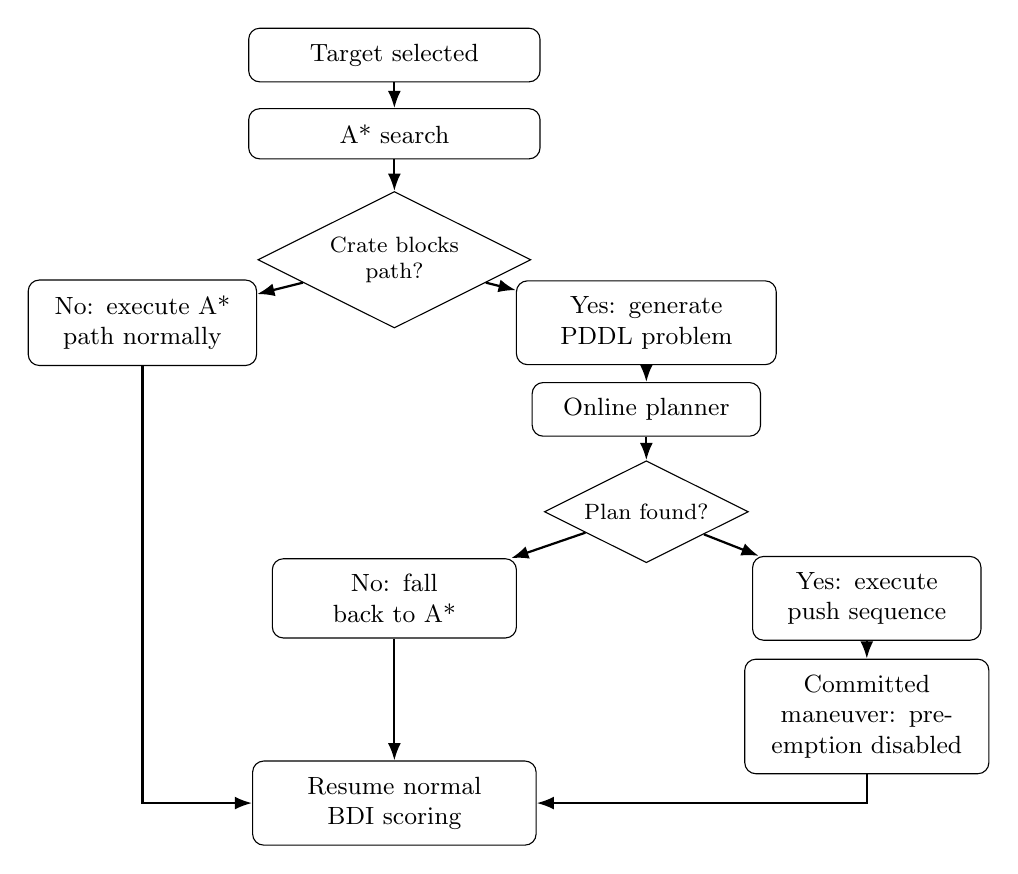
\begin{tikzpicture}[font=\footnotesize]
\node[box] (target) at (4.3,6.6) {Target selected};
\node[box] (astar) at (4.3,5.6) {A* search};
\node[decision,text width=2.0cm] (blocked) at (4.3,4) {Crate blocks path?};
\node[box,text width=2.5cm] (continue) at (1.1,3.2) {No: execute A* path normally};
\node[box,text width=2.9cm] (genpddl) at (7.5,3.2) {Yes: generate PDDL problem};
\node[box,text width=2.5cm] (planner) at (7.5,2.1) {Online planner};
\node[decision,text width=1.9cm] (found) at (7.5,0.8) {Plan found?};
\node[box,text width=2.7cm] (fallback) at (4.3,-0.3) {No: fall back to A*};
\node[box,text width=2.5cm] (pushseq) at (10.3,-0.3) {Yes: execute push sequence};
\node[box,text width=2.7cm] (committed) at (10.3,-1.8) {Committed maneuver: preemption disabled};
\node[box,text width=3.2cm] (resumebdi) at (4.3,-2.9) {Resume normal BDI scoring};

\draw[arr] (target) -- (astar);
\draw[arr] (astar) -- (blocked);
\draw[arr] (blocked) -- (continue);
\draw[arr] (blocked) -- (genpddl);
\draw[arr] (genpddl) -- (planner);
\draw[arr] (planner) -- (found);
\draw[arr] (found) -- (fallback);
\draw[arr] (found) -- (pushseq);
\draw[arr] (pushseq) -- (committed);
\draw[arr] (continue.south) -- (1.1,-2.9) -- (resumebdi.west);
\draw[arr] (fallback) -- (resumebdi);
\draw[arr] (committed.south) -- (10.3,-2.9) -- (resumebdi.east);
\end{tikzpicture}
\caption{Crate blocking and PDDL recovery. \texttt{crateBlocksRoute()} double-checks the block
(crate-respecting plan fails, crate-ignoring plan succeeds) before paying the cost of a solver
call; a found plan runs as a committed maneuver immune to preemption.}
\label{fig:pddl-recovery}
\end{figure}

\end{document}
